% Diagram Arsitektur Kerangka Kerja Restorasi Dokumen Berorientasi HTR
% Dual-Modal GAN dengan Diskriminator CNN+LSTM dan Frozen HTR Recognizer

\begin{figure*}[!t]
\centering
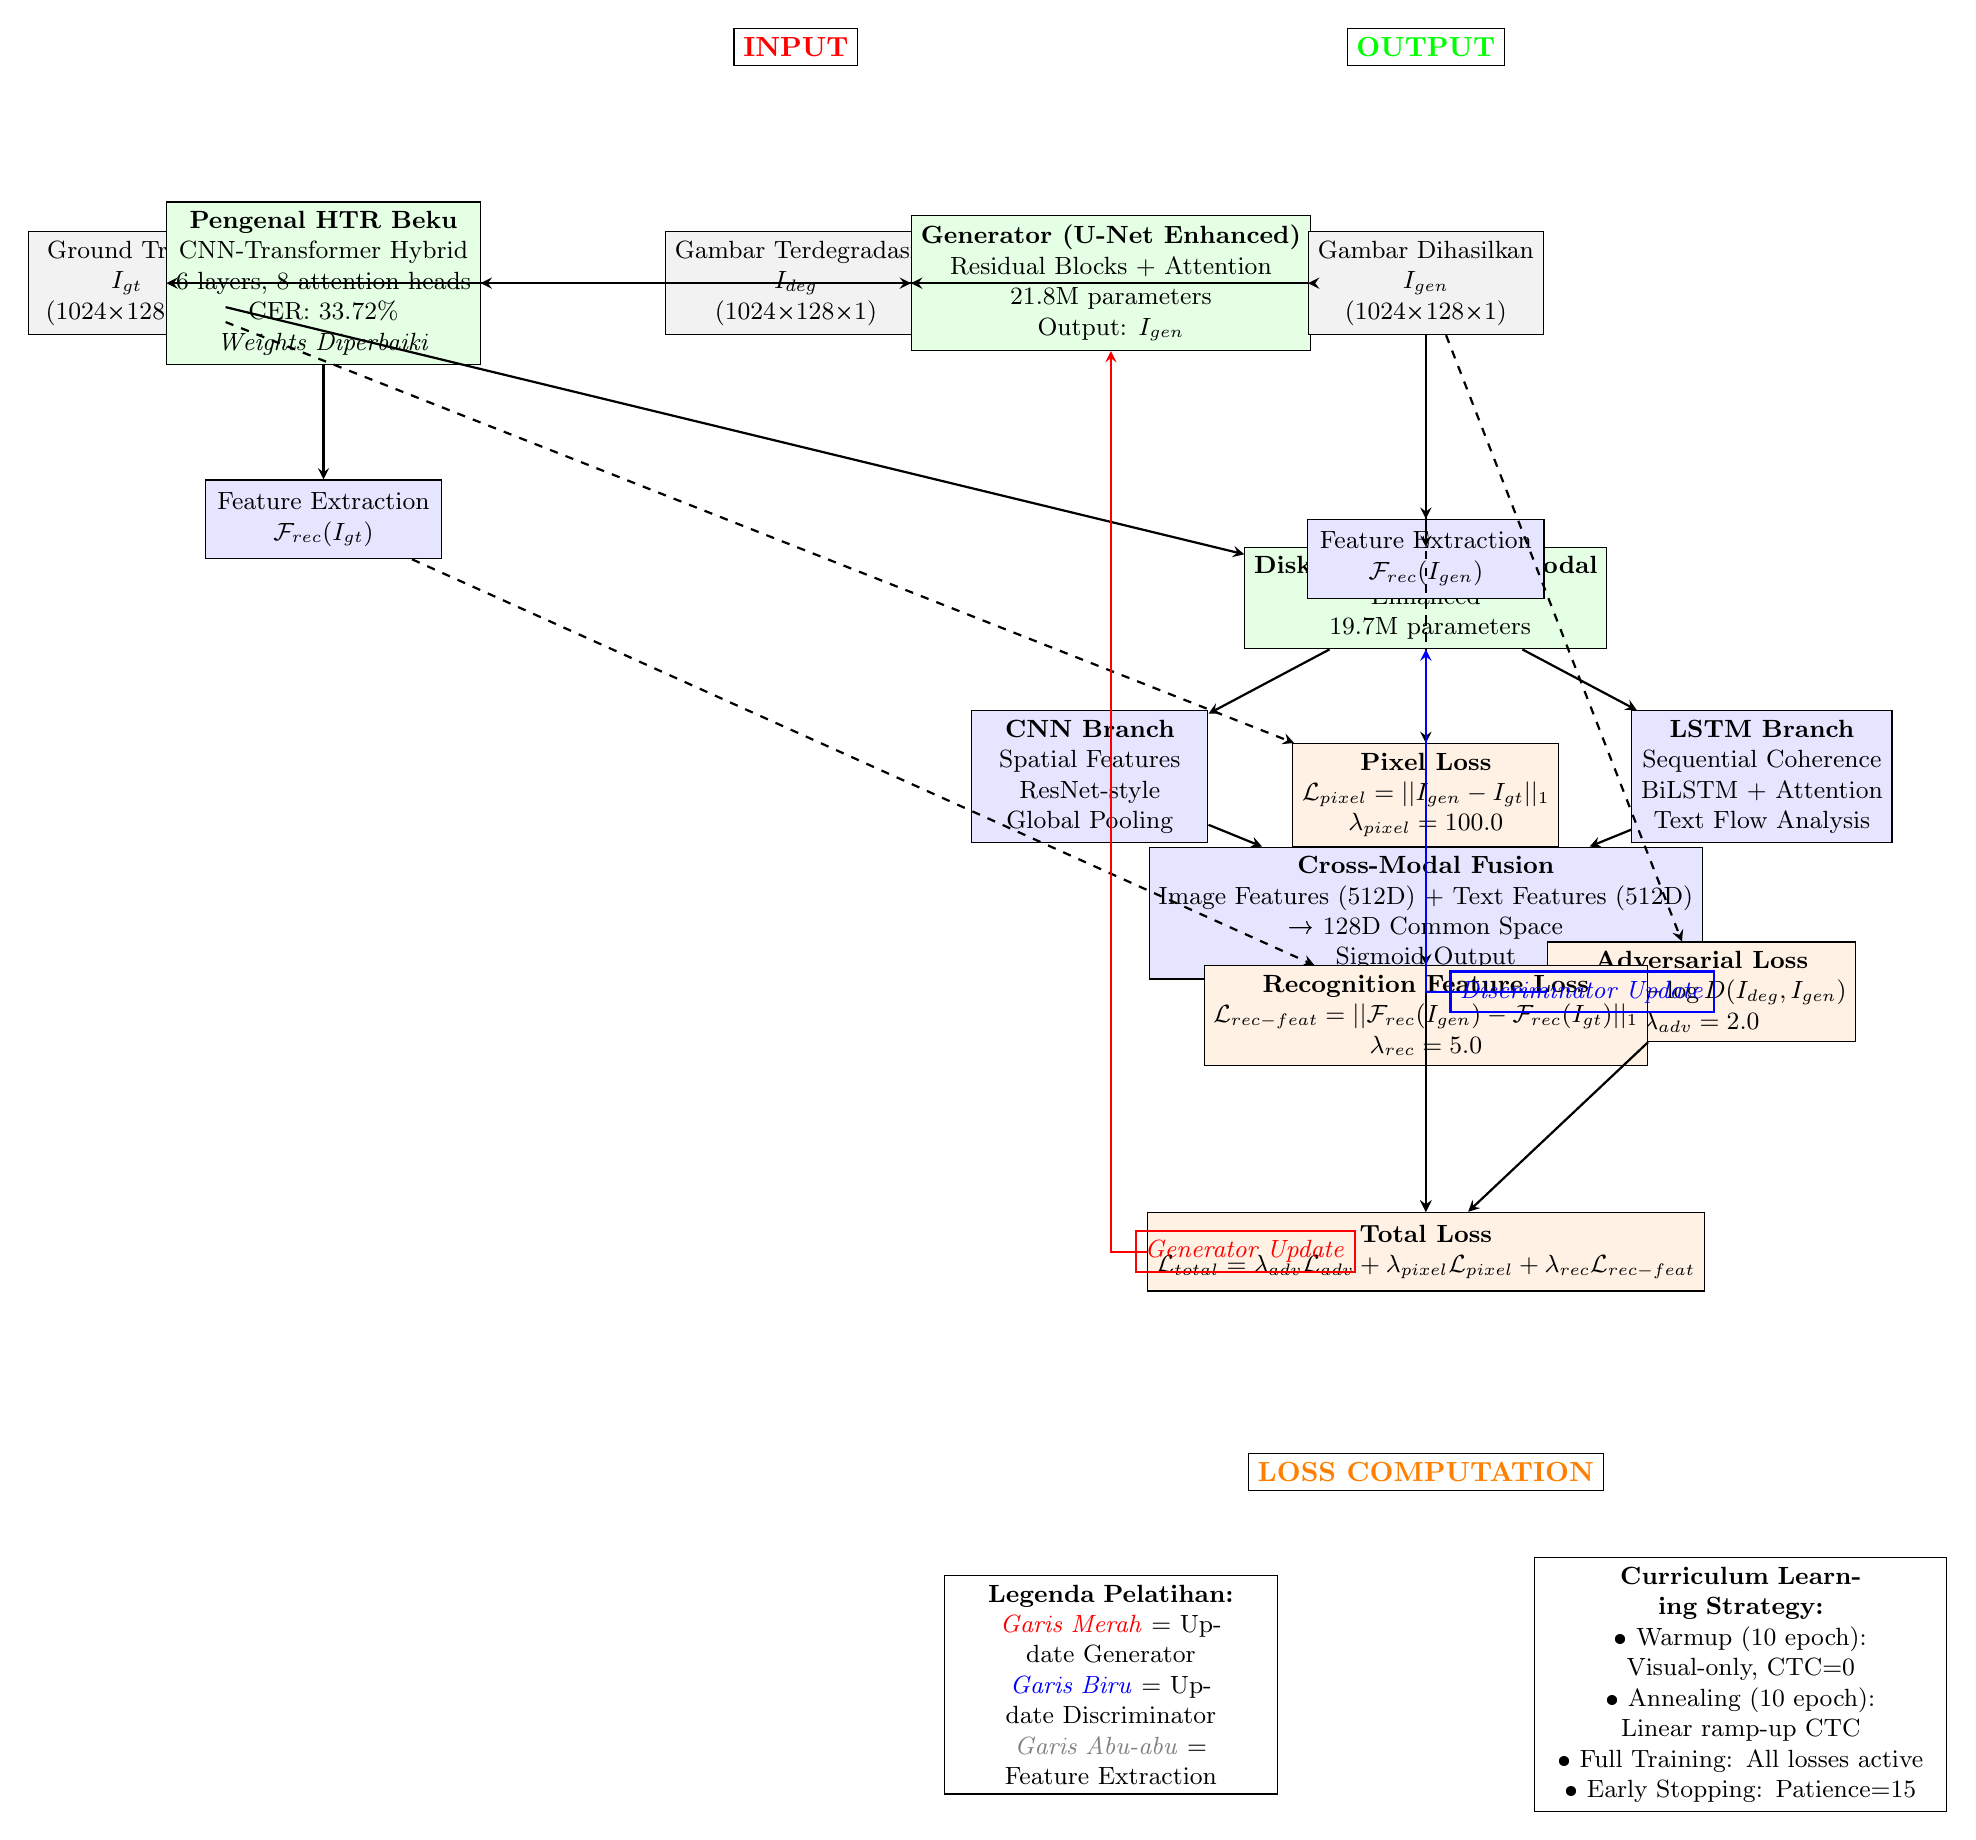
\begin{tikzpicture}[
    node distance=2.5cm,
    font=\small,
    >=stealth,
    every node/.style={rectangle, draw, align=center},
    process/.style={rectangle, draw, fill=blue!10, minimum width=3cm, minimum height=1cm},
    model/.style={rectangle, draw, fill=green!10, minimum width=3.5cm, minimum height=1.2cm},
    loss/.style={rectangle, draw, fill=orange!10, minimum width=3cm, minimum height=1cm},
    data/.style={rectangle, draw, fill=gray!10, minimum width=2.5cm, minimum height=0.8cm},
    arrow/.style={->, thick}
]

    % Input Images
    \node (degraded) [data] {Gambar Terdegradasi \\ $I_{deg}$ \\ (1024×128×1)};
    \node (clean) [data, left of=degraded, xshift=-6cm] {Ground Truth \\ $I_{gt}$ \\ (1024×128×1)};

    % Generator
    \node (generator) [model, right of=degraded, xshift=1.5cm] {\textbf{Generator (U-Net Enhanced)} \\
    Residual Blocks + Attention \\
    21.8M parameters \\
    Output: $I_{gen}$};

    % Generated Image
    \node (generated) [data, right of=generator, xshift=1.5cm] {Gambar Dihasilkan \\ $I_{gen}$ \\ (1024×128×1)};

    % Dual-Modal Discriminator
    \node (discriminator) [model, below of=generated, yshift=-1.5cm] {\textbf{Diskriminator Dual-Modal} \\
    Enhanced \\
    ~19.7M parameters};

    % Discriminator Branches
    \node (cnn_branch) [process, below left of=discriminator, xshift=-2.5cm, yshift=-0.5cm] {\textbf{CNN Branch} \\
    Spatial Features \\
    ResNet-style \\
    Global Pooling};

    \node (lstm_branch) [process, below right of=discriminator, xshift=2.5cm, yshift=-0.5cm] {\textbf{LSTM Branch} \\
    Sequential Coherence \\
    BiLSTM + Attention \\
    Text Flow Analysis};

    % Cross-Modal Fusion
    \node (fusion) [process, below of=discriminator, yshift=-1.5cm] {\textbf{Cross-Modal Fusion} \\
    Image Features (512D) + Text Features (512D) \\
    → 128D Common Space \\
    Sigmoid Output};

    % Frozen HTR Recognizer
    \node (recognizer) [model, left of=generator, xshift=-7.5cm] {\textbf{Pengenal HTR Beku} \\
    CNN-Transformer Hybrid \\
    6 layers, 8 attention heads \\
    CER: 33.72\% \\
    \textit{Weights Diperbaiki}};

    % Feature Extraction from Recognizer
    \node (feat_clean) [process, below of=recognizer, yshift=-0.5cm] {Feature Extraction \\
    $\mathcal{F}_{rec}(I_{gt})$};

    \node (feat_gen) [process, below of=generated, yshift=-1cm] {Feature Extraction \\
    $\mathcal{F}_{rec}(I_{gen})$};

    % Loss Components
    \node (pixel_loss) [loss, below of=feat_gen, yshift=-0.5cm] {\textbf{Pixel Loss} \\
    $\mathcal{L}_{pixel} = ||I_{gen} - I_{gt}||_1$ \\
    $\lambda_{pixel} = 100.0$};

    \node (adv_loss) [loss, below of=discriminator, xshift=3.5cm, yshift=-2.5cm] {\textbf{Adversarial Loss} \\
    $\mathcal{L}_{adv} = -\log D(I_{deg}, I_{gen})$ \\
    $\lambda_{adv} = 2.0$};

    \node (rec_feat_loss) [loss, below of=pixel_loss, yshift=-0.3cm] {\textbf{Recognition Feature Loss} \\
    $\mathcal{L}_{rec-feat} = ||\mathcal{F}_{rec}(I_{gen}) - \mathcal{F}_{rec}(I_{gt})||_1$ \\
    $\lambda_{rec} = 5.0$};

    \node (total_loss) [loss, below of=rec_feat_loss, yshift=-0.5cm] {\textbf{Total Loss} \\
    $\mathcal{L}_{total} = \lambda_{adv}\mathcal{L}_{adv} + \lambda_{pixel}\mathcal{L}_{pixel} + \lambda_{rec}\mathcal{L}_{rec-feat}$};

    % Training Flow Arrows
    \draw [arrow] (degraded) -> (generator);
    \draw [arrow] (clean) -> (generator);
    \draw [arrow] (generator) -> (generated);

    \draw [arrow] (clean) -> (discriminator);
    \draw [arrow] (generated) -> (discriminator);
    \draw [arrow] (discriminator) -> (cnn_branch);
    \draw [arrow] (discriminator) -> (lstm_branch);
    \draw [arrow] (cnn_branch) -> (fusion);
    \draw [arrow] (lstm_branch) -> (fusion);

    \draw [arrow] (clean) -> (recognizer);
    \draw [arrow] (generated) -> (recognizer);
    \draw [arrow] (recognizer) -> (feat_clean);
    \draw [arrow] (generated) -> (feat_gen);

    % Loss Computation Arrows
    \draw [arrow, dashed] (clean) -> (pixel_loss);
    \draw [arrow, dashed] (generated) -> (pixel_loss);
    \draw [arrow, dashed] (generated) -> (adv_loss);
    \draw [arrow, dashed] (feat_clean) -> (rec_feat_loss);
    \draw [arrow, dashed] (feat_gen) -> (rec_feat_loss);
    \draw [arrow] (pixel_loss) -> (total_loss);
    \draw [arrow] (adv_loss) -> (total_loss);
    \draw [arrow] (rec_feat_loss) -> (total_loss);

    % Training Update Arrows
    \draw [arrow, red, thick] (total_loss) -| node[anchor=west, xshift=0.3cm] {\textit{Generator Update}} (generator);
    \draw [arrow, blue, thick] (adv_loss) -| node[anchor=west, xshift=0.3cm] {\textit{Discriminator Update}} (discriminator);

    % Labels
    \node [above of=degraded, yshift=0.5cm, font=\bfseries, text=red] {INPUT};
    \node [above of=generated, yshift=0.5cm, font=\bfseries, text=green] {OUTPUT};
    \node [below of=total_loss, yshift=-0.3cm, font=\bfseries, text=orange] {LOSS COMPUTATION};

    % Training Legend
    \node [below of=total_loss, yshift=-3cm, xshift=-4cm, text width=4cm, font=\small] {
        \textbf{Legenda Pelatihan:} \\
        \textcolor{red}{\textit{Garis Merah}} = Update Generator \\
        \textcolor{blue}{\textit{Garis Biru}} = Update Discriminator \\
        \textcolor{gray}{\textit{Garis Abu-abu}} = Feature Extraction
    };

    % Curriculum Learning Info
    \node [below of=total_loss, yshift=-3cm, xshift=4cm, text width=5cm, font=\small] {
        \textbf{Curriculum Learning Strategy:} \\
        • Warmup (10 epoch): Visual-only, CTC=0 \\
        • Annealing (10 epoch): Linear ramp-up CTC \\
        • Full Training: All losses active \\
        • Early Stopping: Patience=15
    };

\end{tikzpicture}

\caption{Gambaran kerangka kerja restorasi dokumen berorientasi HTR yang diusulkan dengan diskriminator dual-modal dan integrasi pengenal yang dibekukan. Arsitektur terdiri dari Generator U-Net Enhanced, Diskriminator Dual-Modal (CNN+LSTM), dan Pengenal HTR Beku. Pelatihan menggunakan strategi curriculum learning dengan multi-component loss function.}
\label{fig:architecture_overview}
\end{figure*}
